\documentclass[11pt,a4paper,headsepline]{scrartcl}
\usepackage[utf8]{inputenc}
\usepackage[T1]{fontenc}
\usepackage[ngerman]{babel}
\usepackage{amsmath}
\usepackage{amsthm}
\usepackage{amssymb}
\usepackage{amsfonts}
\usepackage[scaled]{helvet}
\usepackage{amssymb}
\usepackage{multirow}
\usepackage{textcomp}
\usepackage{graphicx}
\usepackage{paralist}
\usepackage{textcomp}
\usepackage{pdflscape} 
\usepackage{marvosym}
\usepackage{float}
\usepackage{siunitx}
\usepackage[siunitx,european,cuteinductors,smartlabels]{circuitikz}
\usepackage{fancyhdr}
\usepackage{pgfplots}
\usepackage{sansmath}
\usetikzlibrary{shapes.geometric}
\usepackage{wasysym}
\usepackage[nix]{optional}
\usepackage{listings}
\lstset{
commentstyle=\color{green!50!black}}

\usetikzlibrary{calc}


%\theoremstyle{definition}
\newtheorem{aufgabe}{Aufgabe}
\newtheorem{loesung}{L\"osung}
\newcommand{\Var}{\operatorname{Var}}
\newcommand{\D}{\operatorname{d}}
\newcommand{\mum}{\operatorname{\mu m}}
\newcommand{\E}{\operatorname{E}}
\newcommand{\var}{\operatorname{var}}
\newcommand{\Id}{\operatorname{Id}}
\newcommand{\rg}{\operatorname{rg}}



\renewcommand*\familydefault{\sfdefault}
%\renewcommand{\arraystretch}{1.1}


\KOMAoptions{parskip=half,DIV=15,fontsize=11pt}
\unitlength1cm
\newif\ifuelsg %als slides
%\uelsgtrue
\uelsgfalse
\newif\ifnotuelsg
\ifuelsg\notuelsgfalse\else\notuelsgtrue\fi

\title{Praktikum ``Zustandsbeobachter''}
\date{}
\makeatletter
\let\Title\@title
\let\Author\@author
\makeatother
\pagestyle{fancy}
\fancyhead[L]{Prof. Dr. Raphael Pfaff}
\fancyhead[R]{85745: Energieeffiziente Antriebsregelung}
\fancyfoot[L]{Datei: \jobname}
\fancyfoot[R]{Datum: \today
\begin{picture}(0,0)(0,0)\put(.5,0){
\includegraphics[height=5cm]{fh_logo}}\end{picture}}


\begin{document}

\maketitle
\thispagestyle{fancy}
\vspace{-2cm}
% \hyphenation{Abwei-chungen}

\section*{Kalman Filter}
\begin{aufgabe}[Funktionsweise und Parameter des Kalman Filters]
\label{Task:KF}
Nutzen Sie das auf Ilias bereitgestellte Skript ``P2KalmanFilter.sce'' um die Zustandssch\"atzung eines linearen Systems durchzuf\"uhren. Dokumentieren Sie Ihre Beobachtungen (wo n\"otig mit Grafikausgabe) in einem formlosen Dokument. 

Variieren Sie (jeweils unab\"angig)
\begin{itemize}
	\item die Rauschamplitude,
	\item das Eingangssignal,
	\item die Systemparameter,
	\item die Initialisierung von
	\begin{itemize}
		\item Startzustand und
		\item $R_{w}$-Matrix.
	\end{itemize}
\end{itemize}
F\"uhren Sie weiterhin zwischen Systemsimulation und Kalman Filter eine kleine St\"orung der $A$-Matrix ein.

\small
\lstinputlisting[language=Scilab]{../Solutions/SolutionP2KalmanFilter.sce}
\end{aufgabe}
\vspace{0.5cm}

\opt{loesung}{
\begin{loesung}[Skript zur L\"osung der Aufgaben \ref{Task:KF}] $ $ \\
Explorative Aufgabe, keine L\"osung vorgegeben.
\end{loesung}
}

\newpage
\normalsize
\begin{aufgabe}[Luenberger-Beobachter in Scilab]
\label{Task:Luenberger}
Erg\"anzen Sie das System-Modell aus dem ersten Praktikum um einen Luenberger-Beobachter zur Zustandssch\"atzung. Beachten Sie folgende Punkte:
\begin{itemize}
	\item Basis der Sch\"atzung ist das Ausgangssignal des Systems, versehen mit additivem wei{\ss}en Rauschen.
	\item Das Rauschsignal importieren Sie mittels eines ``fromWorkspace''-Blocks.
	\item Zeichnen Sie folgenden Zust\"ande auf:
	\begin{itemize}
		\item Eingangssignal $u$
		\item Wahre Zust\"ande $x_{1}$, $y_{0} = x_{2}$
		\item Gesch\"atzte Zust\"ande $\hat{x}_{1}$, $\hat{x}_{2}$
		\item Gemessenes (verrauschtes) Ausgangssignal $y_{n}$
	\end{itemize}
	\item Stellen Sie in je einem Plot gegen\"uber:
	\begin{itemize}
		\item $u$, $y_{0}$, $y_{n}$
		\item $x_{1}$, $\hat{x}_{1}$
		\item $x_{2}$, $\hat{x}_{2}$
		\end{itemize}
	\item W\"ahlen Sie $L = \left(0{,}2 \; 0{,}1\right)^T$
\end{itemize}
\begin{center}
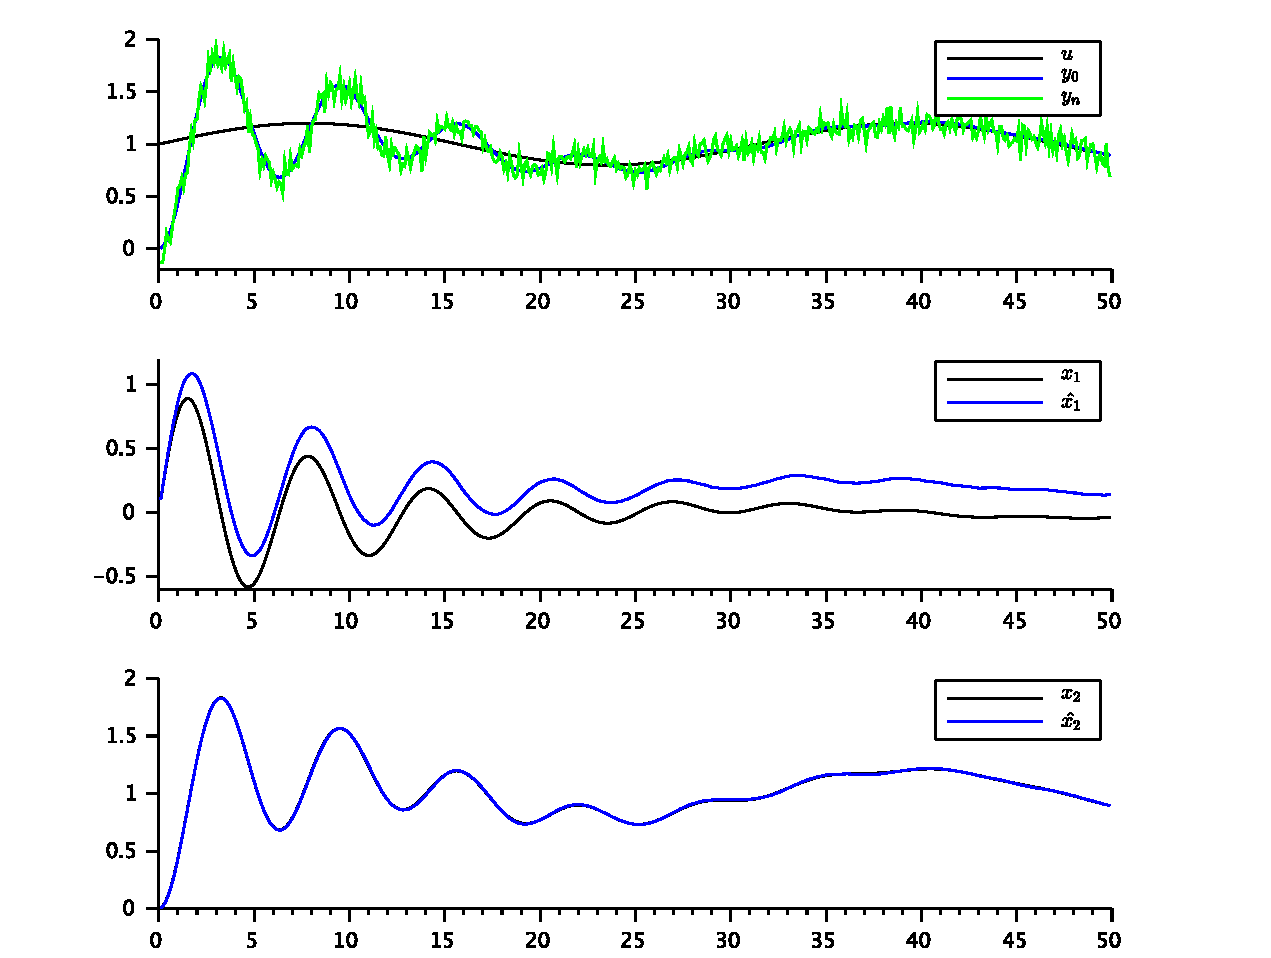
\includegraphics[width = 0.8\textwidth]{P22Output}
\end{center}
\end{aufgabe}

\opt{loesung}{
\newpage
\begin{loesung}[Skript zur L\"osung der Aufgaben \ref{Task:Luenberger}] $ $ \\
\lstinputlisting[language=Scilab]{../Loesungen/151229P22.sce}

\begin{figure}[htbp]
\begin{center}
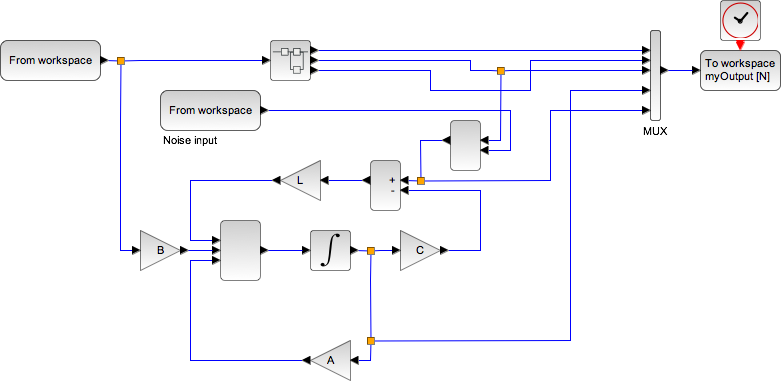
\includegraphics[width = 0.9\textwidth]{../Loesungen/P22Scicos}
\caption{XCos Blockdiagramm}
\label{default}
\end{center}
\end{figure}
\end{loesung}
}


\end{document}